\documentclass{article}
\usepackage{amsmath}
\usepackage{enumitem}
\usepackage{graphicx}
\usepackage{framed}
\usepackage{listings}
\usepackage{pdfpages}
\usepackage{caption}
\usepackage{subcaption}
\usepackage[utf8]{inputenc}
\usepackage{minted}
\usepackage{placeins}


\title{Chapter 3 Group Assignment}
\author{Will Rudisill, Tate Meehan, Arash Modaresi Rad}
\usepackage[utf8]{inputenc}
\begin{document}
\maketitle

\section*{Problem 4}
\subsection*{a.}
For the G matrix containing the row and column scans only, the dimensions are $m=324$, $n=256$ and the rank is 31. For the G  matrix containing all of the scans, the dimensions are $m=94$, $n=256$ and the rank is 87. 
\subsection*{b.}
\subsubsection*{Part 1} \textbf{State and discuss the general solution and data fit significance of the elements and dimensions of the data and model null spaces.} \\
The model (N(G)) and data (N(G$^T$)) provide vital information about the behavior of the linear system. If only the model null space is non trivial (it contains vectors other than the zero vector), then the data can be fit exactly, but there are an infinite number of solutions that fit. In this case the solution m is equivalent to m = m$_\dagger$ + m$_0$ where m$_0$ is some arbitrary vector from the model nullspace. The general pseudoinverse solution has the convenient property that m$_\dagger$ is always the minimum length least squares solution ($\Vert m \Vert_2^2 \leq \Vert m_\dagger \Vert$). 
When the data nullspace N(G$^T$) is also non-trivial, then the above holds true, though additionally the data vector d does not lie within the R(G). The Gm$_\dagger$ also yields the point in R(G) that is the closest to d in the least squares sense. 
The dimensions of the data null space vector are given by m-p, since there there are m-p columns of U$_0$ that form the the orthonormal basis for the null space N(G$^T$). Likewise, the dimension of the model nullspace N(G) are given by n-p, since there are n-p columns of V$_0$ that form the orthonormal basis for N(G). For this problem, dimensions of A,B yield:
\begin{table}[h!]
    \centering
    \begin{tabular}{|c|c|c|c|c|}
        \hline
         Case & dim(G) & p & dim(N(G)) & dim(N(G$^T$)) \\
        \hline
        A & 32 , 256 & 31 & 1 & 225 \\ 
        B & 94 , 256 & 87 & 7 & 162 \\ 
        %  & A & 32, 256 & \\
        %  & B & 94, 256 & 
        \hline
    \end{tabular}
    \caption{The dimensions, truncation value, and model and data nullspace dimensions for the tomography problem for raypath cases A and B.}
    \label{tab:my_label}
\end{table}
Since in each case p $<$ m and p $<$ n, neither the data nor model null spaces are non-trivial. Consequently we have a case where the pseudoinverse produces a solution that minimizes both the two norm of the residual vector and the two norm of the model parameter vector (so, the pseudo inverse solution provides the least squares and the minimum length least squares solution).
Figure \ref{nullspace} displays one such model null space vector that satisfies Gm=d=0 exactly for A and B. The sums of the rows, the columns, and the diagonal elements are 0 respectively. 

\begin{figure}[ht!]
    \centering
    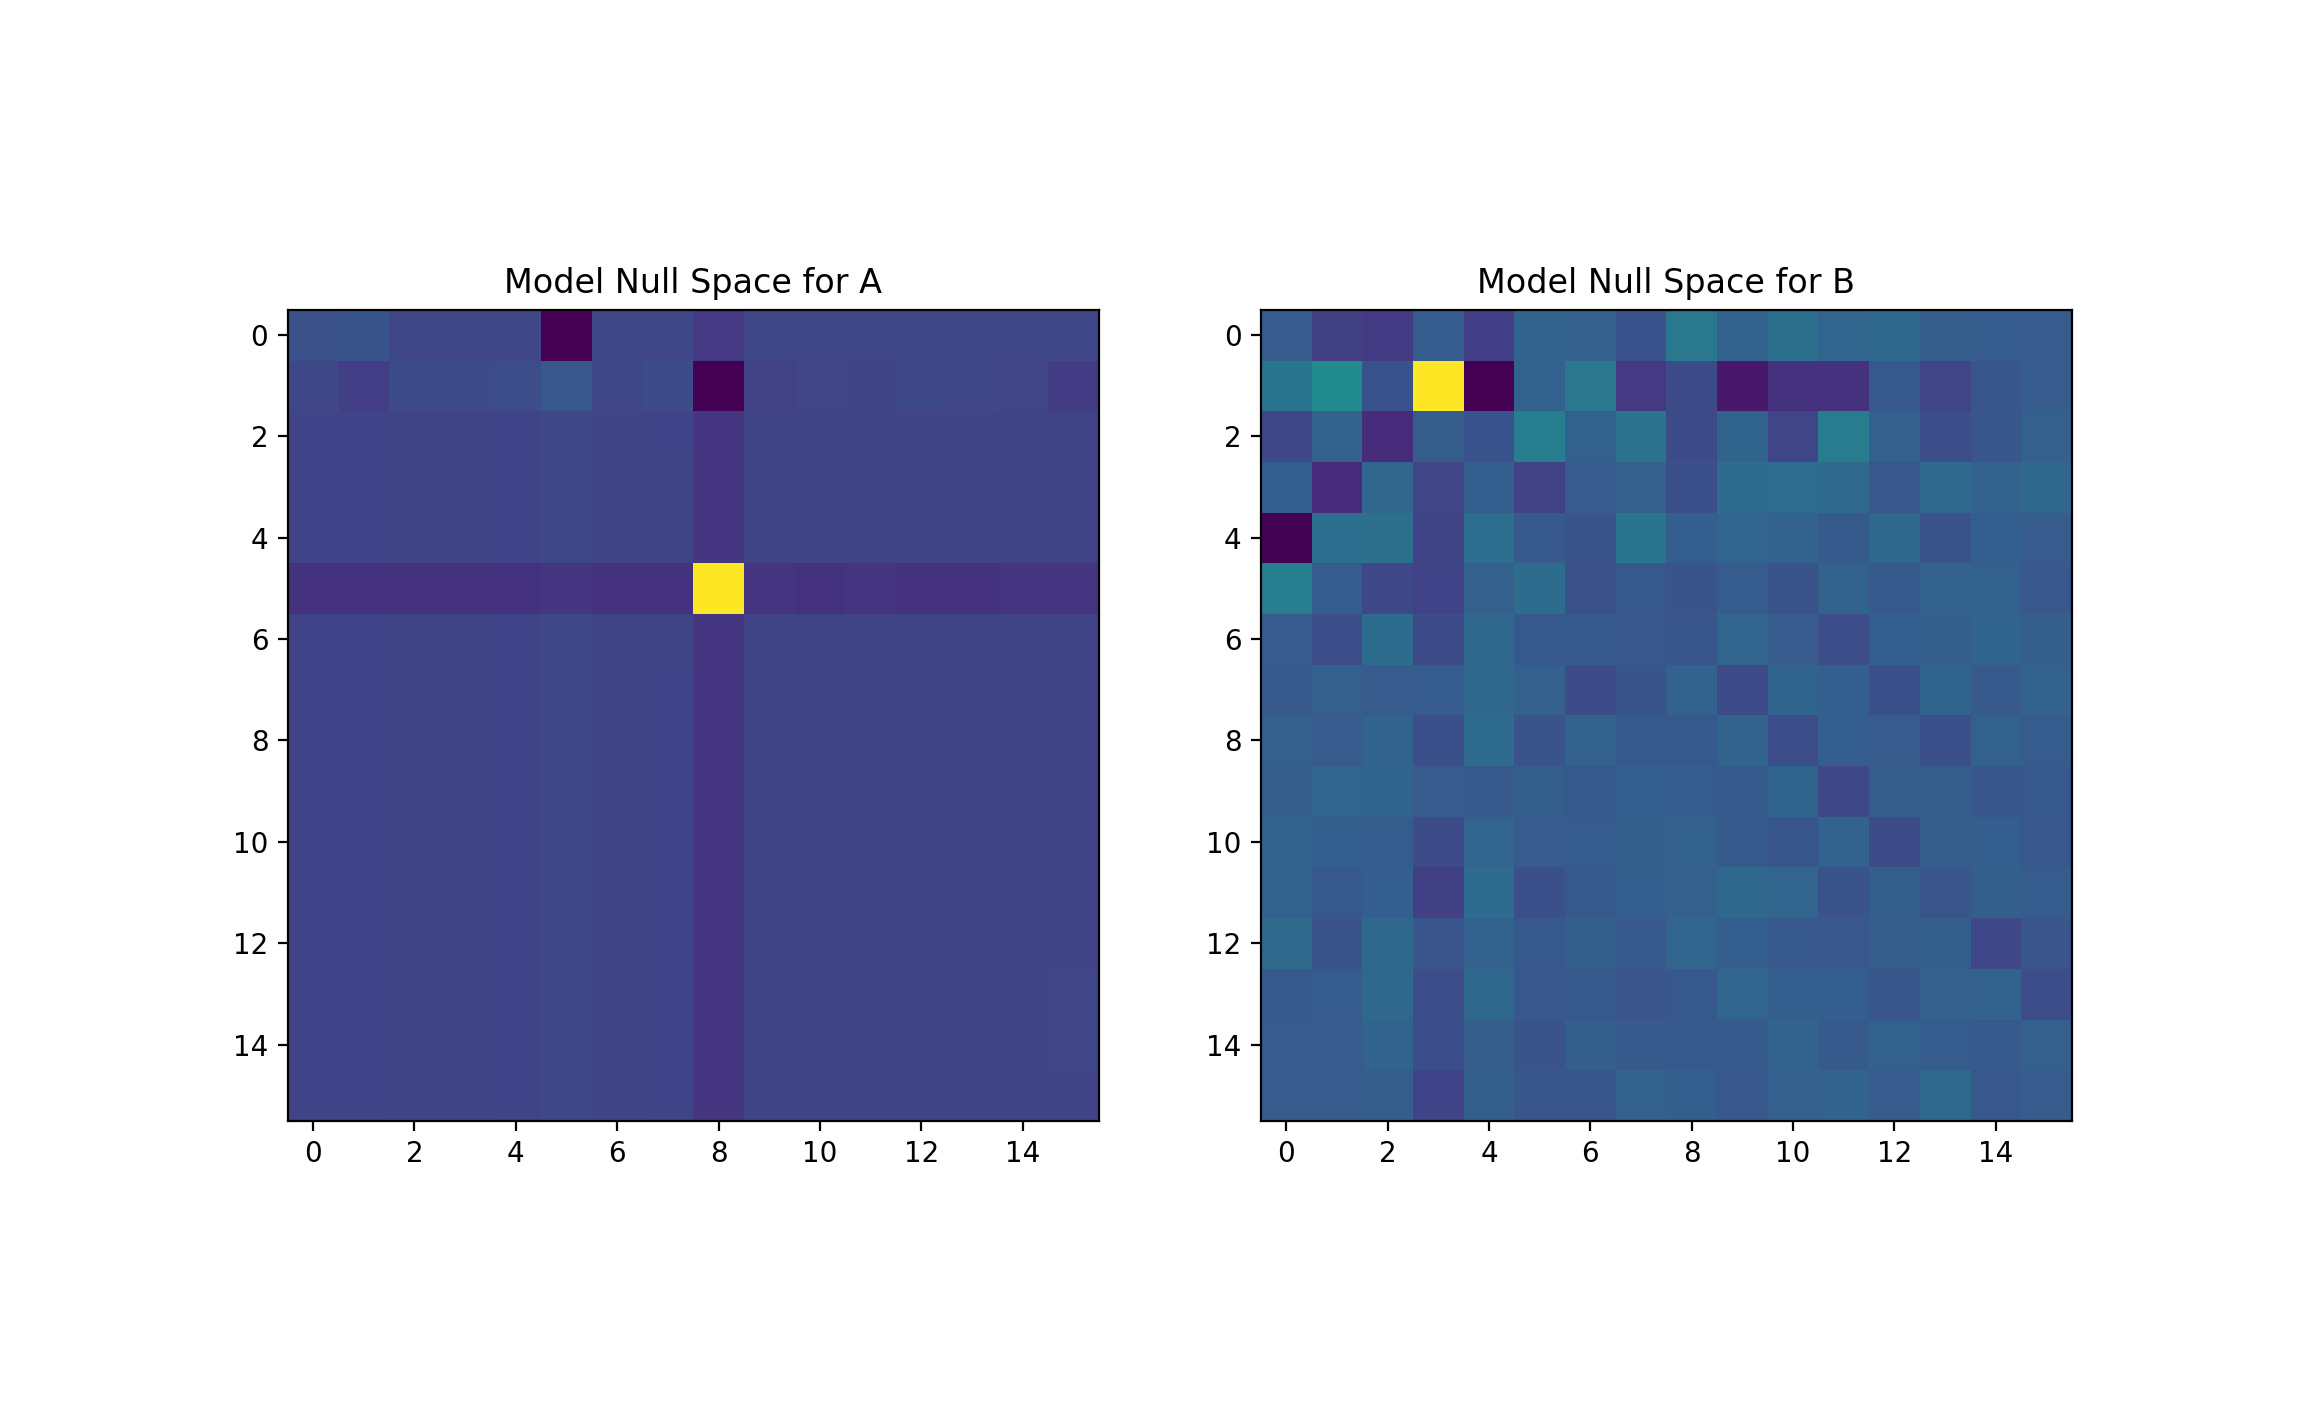
\includegraphics[width=4in]{Nullspace.png}
    \caption{Nullspaces corresponding with V$_{p+1}$ for models A and B}
    \label{nullspace}
\end{figure}

\subsubsection*{Part 2}\textbf{Show the model resolution by contouring or otherwise displaying the 256 diagonal elements of the model resolution matrix, reshaped into an appropriate 16 by 16 grid. Note if there are any model parameters that have perfect resolution.}

Figure \ref{resolution} shows the reshaped model resolution matrices for A and B. The A resolution matrix has a much more uniform resolution (approximately 1.26) whereas the B matrix a more heterogeneous resolution matrix. The corner elements of the resolution matrix for B are 1, which means that they are well resolved. 

\begin{figure}[h!]
    \centering
    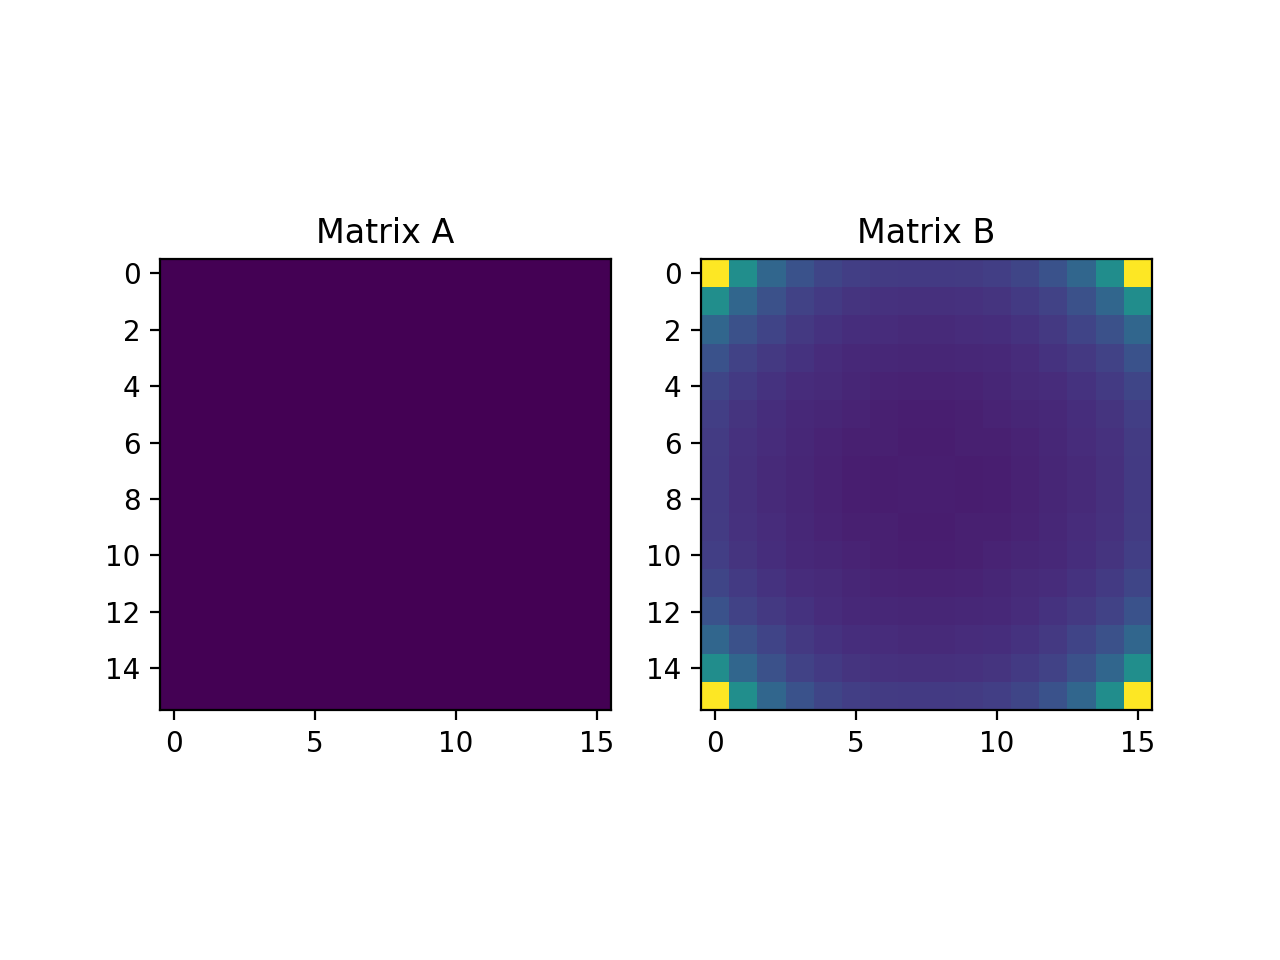
\includegraphics[width=4.5in]{resolution_matrices.png}
    \caption{Model resolution matrices for the A and B forward operators. The left matrix has a nearly uniform resolution of approximately 1.26 for each parameter. The corner elements of B have a resolution of exactly 1}
    \label{resolution}
\end{figure}

\subsection*{c.}
Figure \ref{slowness imagel} shows the slowness perturbations for models A and B. Both have a similar magnitude of perturbation slownesses. The darker areas are zones of lesser slowness (i.e., greater velocity). These can correspond with geologic features (such as dinosaur bones). 

\begin{figure}[p]
    \centering
    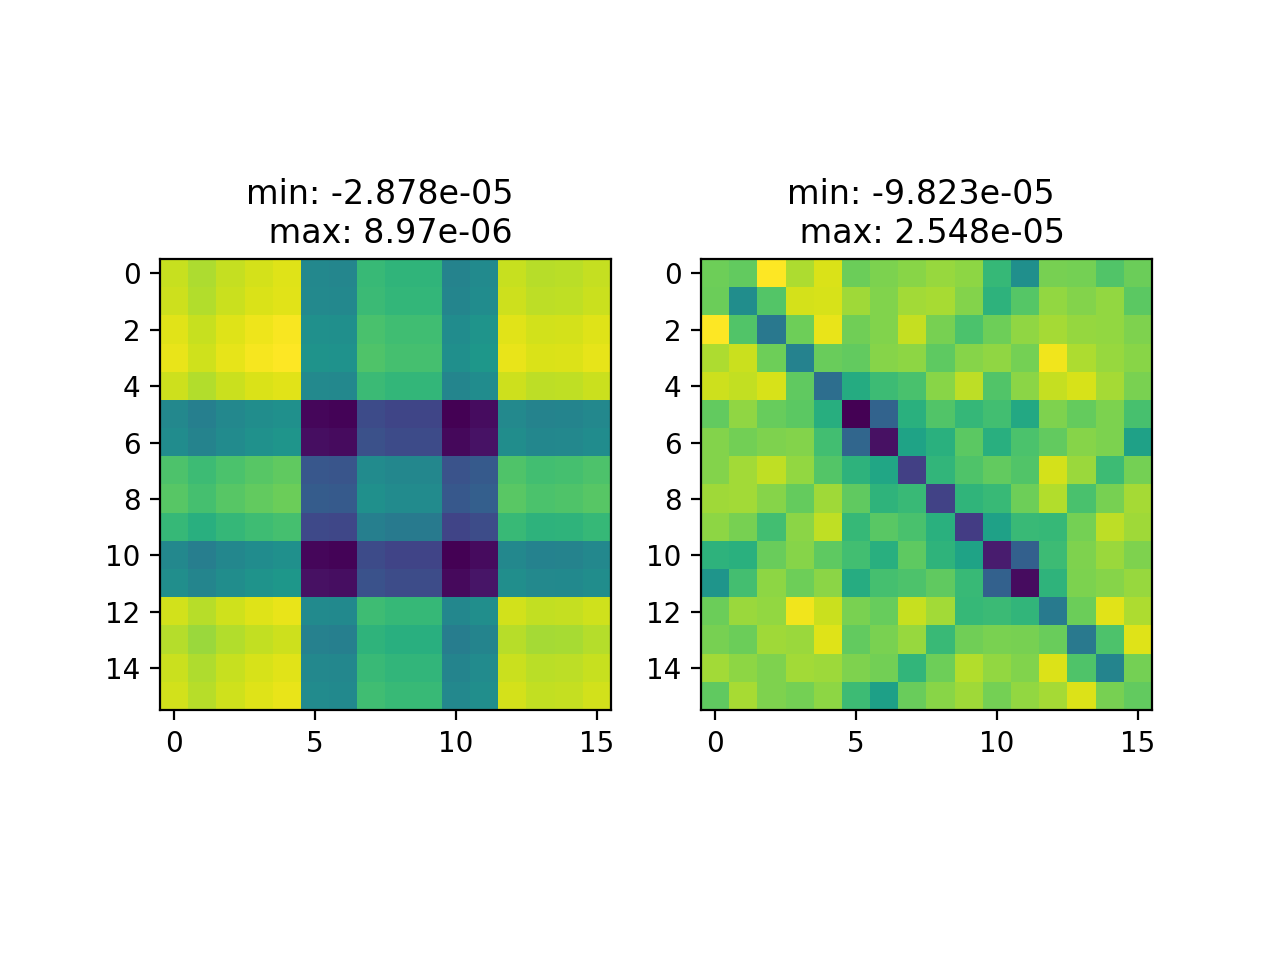
\includegraphics[width=4.5in]{slowness_plots.png}
    \caption{Slowness perturbations plotted for case A (left) and B (right)}
    \label{slowness imagel}
\end{figure}


\newpage
\subsection*{d.}
One can create a different model by adding a linear combination of an element of the model nullspace to the m$_\dagger$ solution, since this vector will satisfy Gm=d=0. An example of such a 'wild model' is given by Figure \ref{Wild}
\begin{figure}[p]
    \centering
    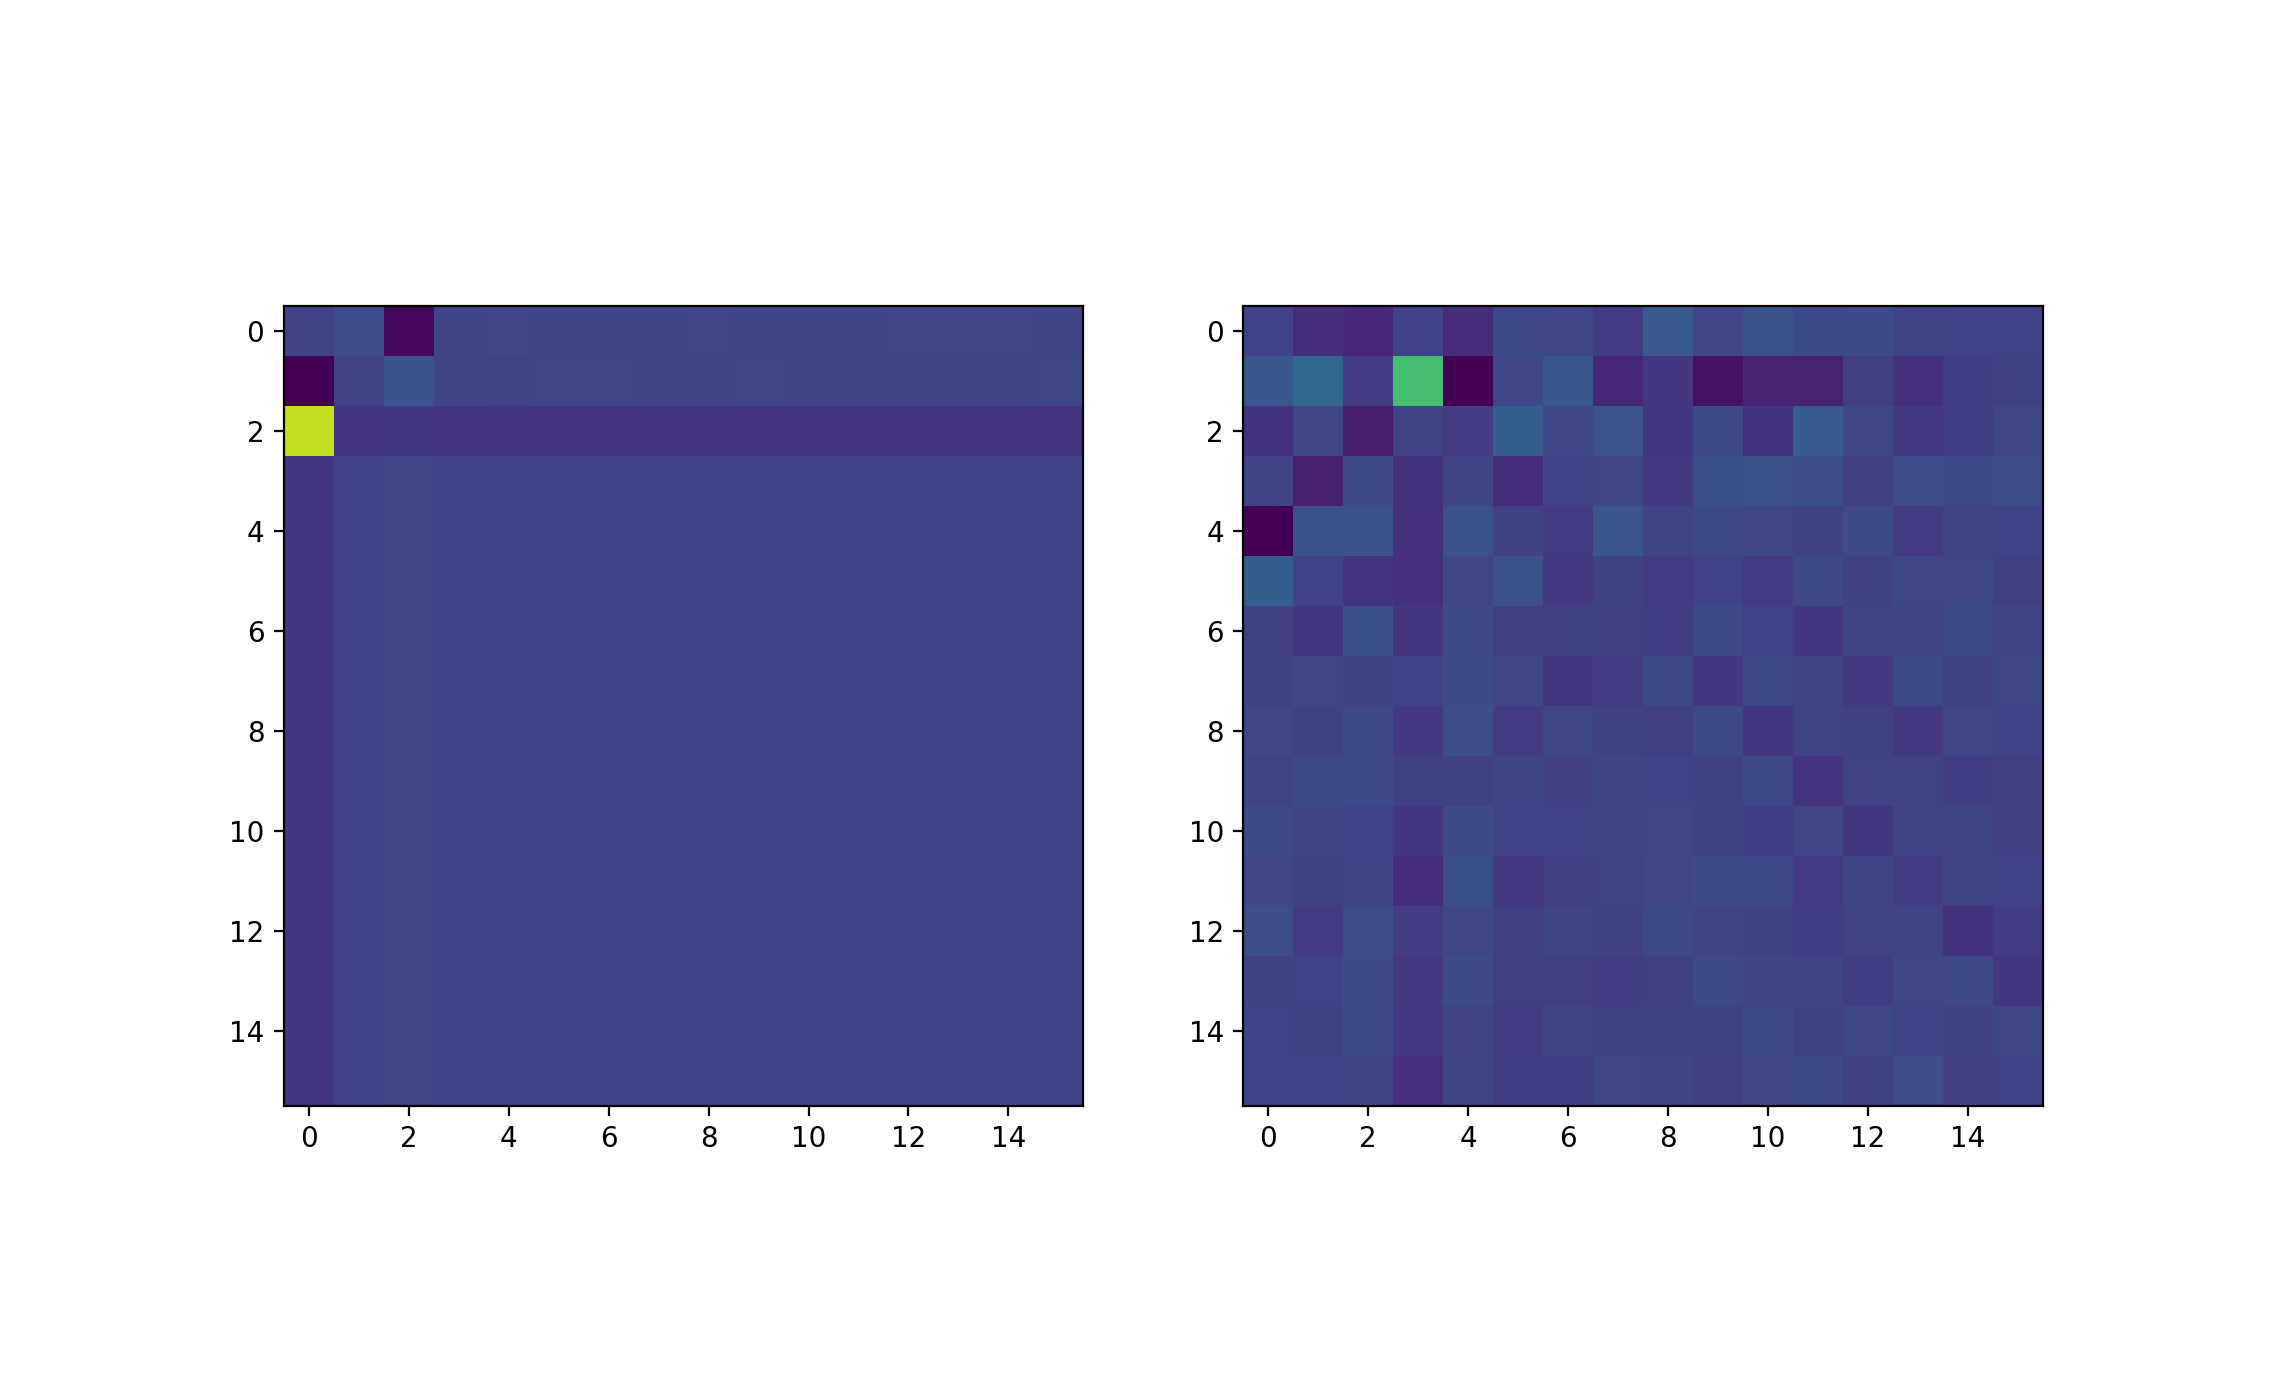
\includegraphics[width=4.5in]{wildplot.png}
    \caption{A "Wild Model" result}
    \label{Wild}
\end{figure}



\newpage

\section*{Problem 5}
\subsection*{a}
The G matrix set up by solving the collocation is shown by Figure \ref{Gmat5}. 

\begin{figure}[hb!]
    \centering
    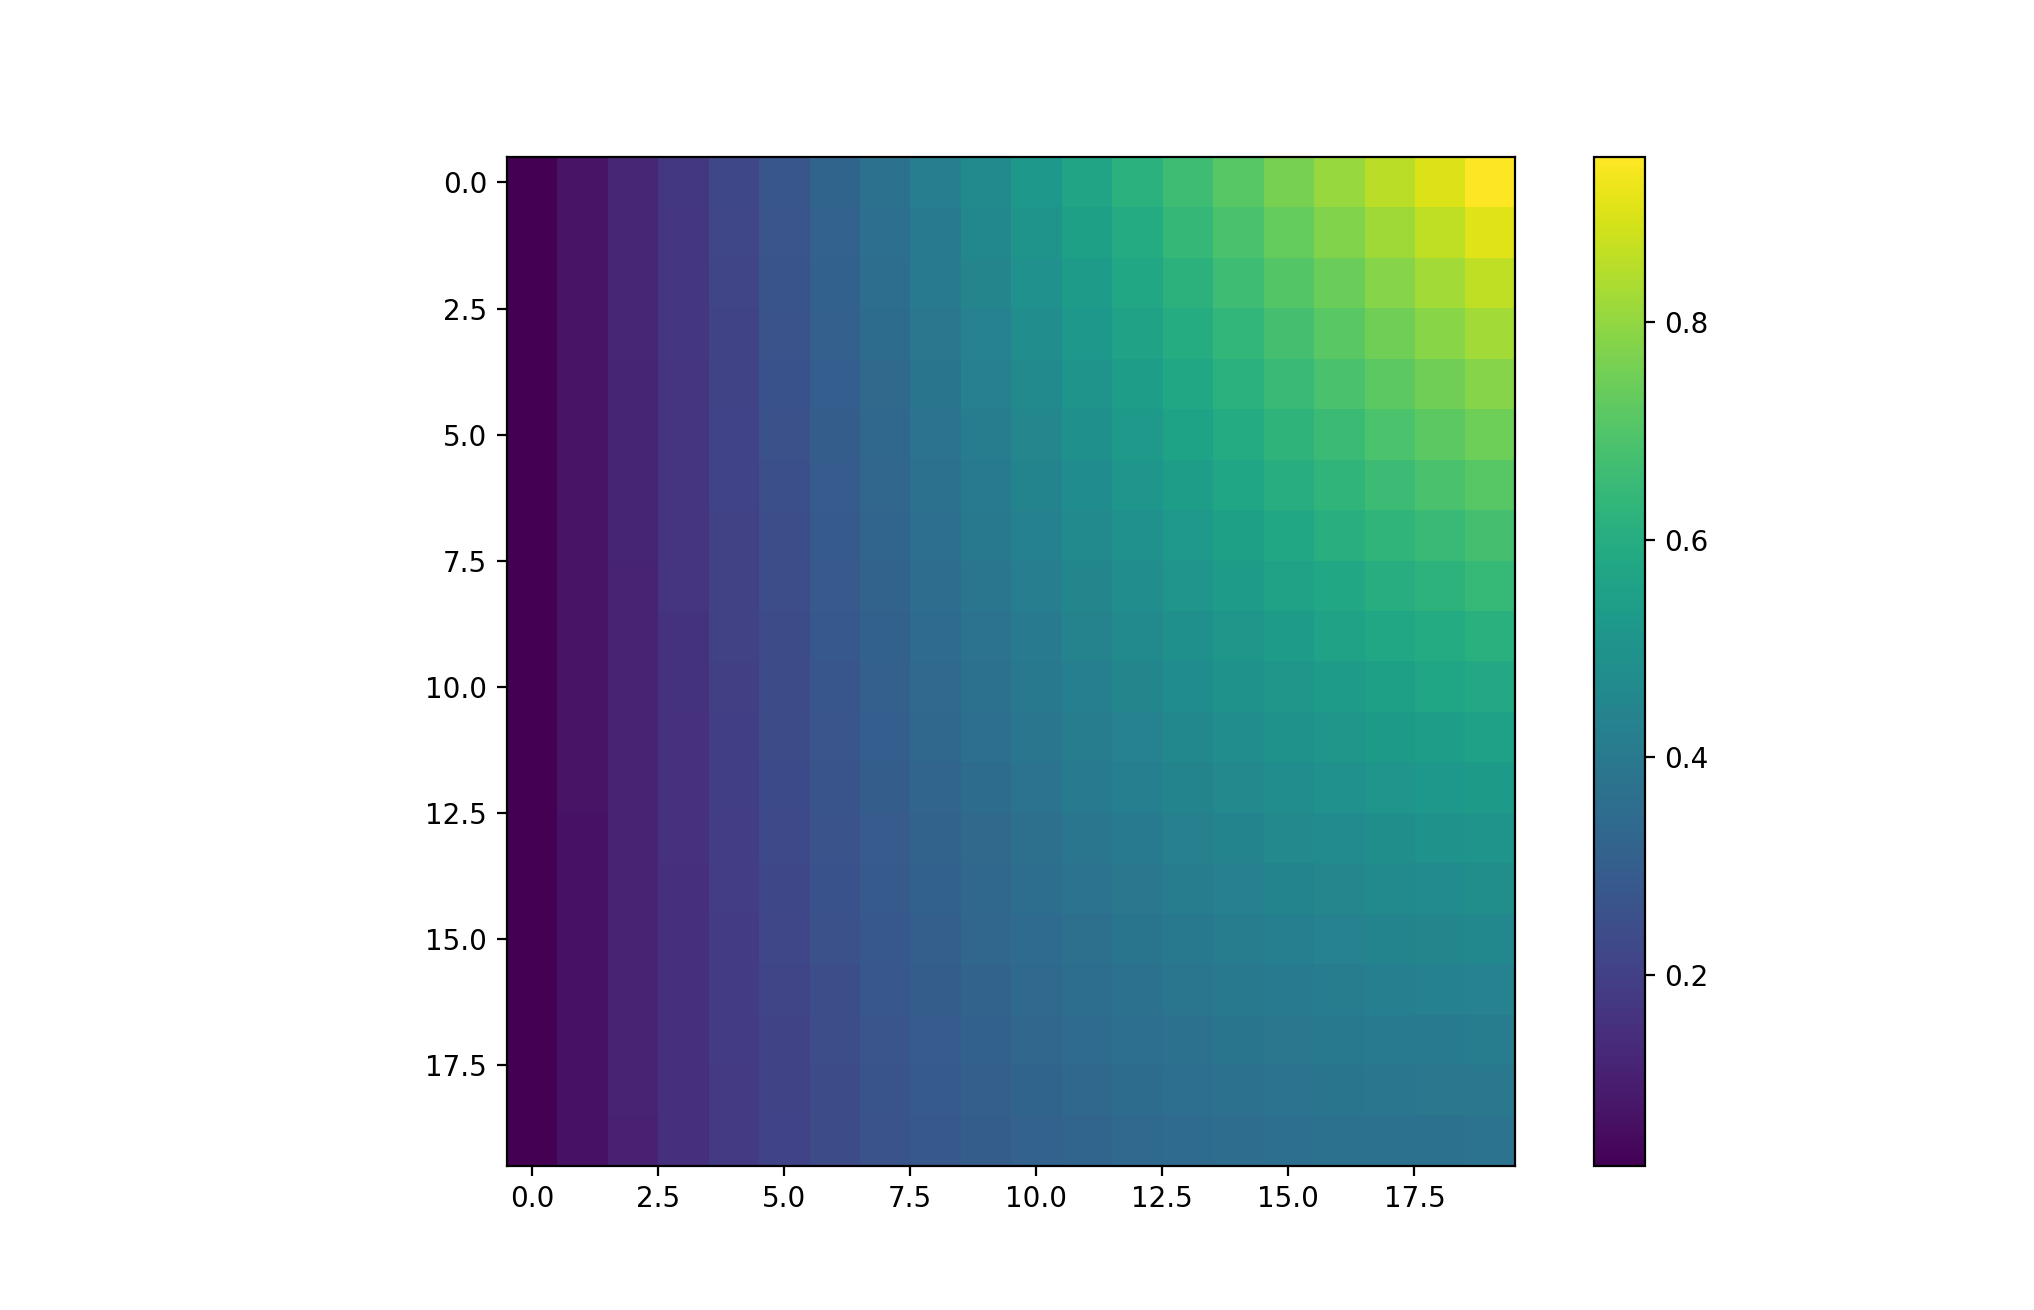
\includegraphics[width=4.5in]{p5G.png}
    \caption{G matrix for simple collocation}
    \label{Gmat5}
\end{figure}

\subsection*{b}
The condition number is very large (effectively infinite), since the matrix is rank deficient and consequently has nearly zero singular values.

\subsection*{c}
The picard ratio is shown in Figure \ref{picard}. Beyond p=8, the singular values become very small. We compute the truncated SVD solution using p=8. 
\begin{figure}
    \centering
    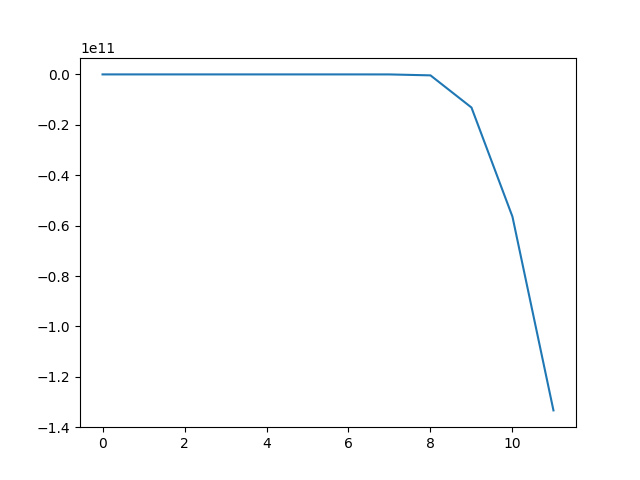
\includegraphics[width=4.5in]{picard.png}
    \caption{Picard Ratio. Singular values beyond p=8 become very small}
    \label{picard}
\end{figure}
The truncated SVD solution dampens out the  sinusoidal pattern that is found in the least squares fit. Each solution gives residuals for each paramter on the order of 1e-6. 

\begin{figure}
    \centering
    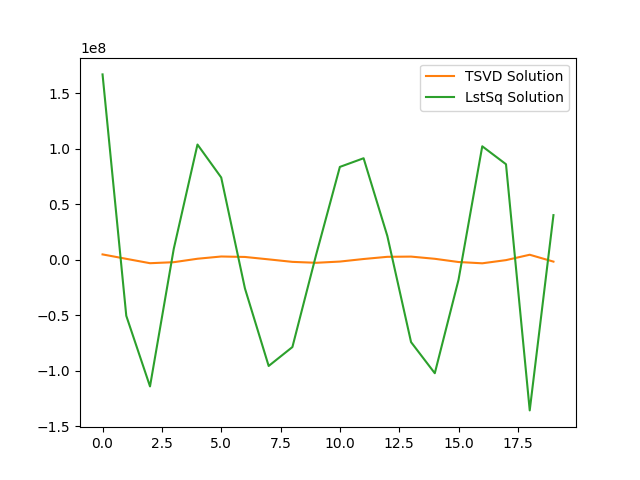
\includegraphics[width=4.5in]{m5solutions.png}
    \caption{lstsq and TSVD solutions for model parameters}
    \label{m5sol}
\end{figure}

\newpage
\section{Appendix--Code}
Code for problem 4
\inputminted{python}{ch3group.py}
Code for problem 5 
\inputminted{python}{ch3group5.py}
\end{document}
